%! Author = Sten
%! Date = 01-11-2020

% Preamble
\documentclass[11pt]{article}

\usepackage[a4paper,margin=2.5cm]{geometry}

% Packages
\usepackage[fleqn]{amsmath}
\usepackage{amsfonts}
\usepackage{graphicx}

\title{Capped hose model: MIP and DP}
\author{David Dekker \and Sten Wessel}
\date{\today}

% Document
\begin{document}
    \maketitle

    Let $G = (V, E)$ be a graph with with edge costs $c\colon E \to \mathbb R_+$, describing a network.
    Let $W \subseteq V$ be a set of terminals.
    Let $\mathcal U$ describe the universe of symmetric demand matrices $(D_{ij})_{i,j \in W}$ (we require that $D_{ii} = 0$ for all $i \in W$), describing the amount of traffic between two terminals.

    We consider a specific universe of demands, called the \emph{capped hose model}.
    We can describe the capped hose model is described by a polytope: each terminal $i$ has maximum capacity $b_i$ (as in the hose model), and additionally there is an upper bound $d_{ij}$ on the demand between terminals $i,j \in W$.
    Hence, we can describe the capped hose polytope $\mathcal H^\text{cap}(b, d)$ as all (symmetric) matrices $(D_{ij})_{i,j \in W}$ for which
    \[
        \begin{split}
            \sum_{j \in W} D_{ij} &\le b_i \qquad&&\forall_{i \in W}, \\
            D_{ij} &\le d_{ij} \qquad&&\forall_{i,j \in \binom W 2}.
        \end{split}
    \]
    Note that setting $d_{ij} = 0$ signals that terminals $i$ and $j$ may not communicate.

    We define a graph $H$ with vertex set the terminals $W$ and edges $W \times W$, weighted with $d_{ij}$.
    We will first derive a compact MIP formulation for general RND problems under the capped hose demand model.
    We will then focus on the case where $H$ is a cycle, i.e.\ terminals are only allowed to communicate with its two direct neighbors in the cycle.
    In this case, a dynamic programming algorithm is suggested by Bosman and Olver, for which it remains open whether it is optimal (for arbitrary $b$ and $d$).

    \section{MIP formulation}
    As for the VPN and generalized VPN problem, we first write the semi-infinite MIP formulation with the row generation subproblems.
    We then use a dualization trick to obtain a compact formulation.

    Let $x_{uv}$ denote the amount of capacity we buy of edge $\{u,v\}$ in the network graph $G$.
    The semi-infinite MIP formulation (the master problem) becomes
    \begin{alignat*}{5}
        \text{minimize}\ && \sum_{uv \in E} c_{uv} \cdot x_{uv} &&& \\
        \text{subject to}\ && x_{uv} &\ge \sum_{ij \in \binom{W}{2}} D_{ij} \cdot (f_{uv}^{ij} + f_{vu}^{ij}) &&\qquad \forall_{uv \in E,\ D \in \mathcal U^*} \\
        && \sum_{uv \in \delta(u)} f_{uv}^{ij} - f_{vu}^{ij} &= \begin{cases}
                                     1 & \text{if $u = i$} \\
                                     -1 & \text{if $u = j$} \\
                                     0 & \text{otherwise}
        \end{cases} &&\qquad \forall_{u \in V,\ ij \in \binom{W}{2}} \\
        && x_{uv} &\in \mathbb{R}_+ &&\qquad \forall_{uv \in E} \\
        && f_{uv}^{ij},\ f_{vu}^{ij} &\in \{ 0, 1 \} &&\qquad \forall_{uv \in E,\ ij \in \binom{W}{2}}
    \end{alignat*}
    where $\mathcal U^* \subseteq \mathcal H^\text{cap}(b, d)$, and is populated by solving the following row generation subproblems (for all $uv \in E$).
    Let $(\tilde x, \tilde f)$ denote the current optimal solution of the master problem.
    \begin{alignat*}{5}
        \text{maximize}\quad && \sum_{ij \in \binom{W}{2}} (\tilde f_{uv}^{ij} + \tilde f_{vu}^{ij}) \cdot D_{ij} &&& \\
        \text{subject to}\quad && D_{ij} &\le d_{ij} &&\qquad \forall_{ij \in \binom W 2} \\
        && \sum_{\substack{j \in W:\\i \neq j}} D_{ij} &\le b_i &&\qquad \forall_{i \in W} \\
        && D_{ij} &\in \mathbb{R}_+ &&\qquad \forall_{ij \in \binom{W}{2}}
    \end{alignat*}
    Let $D^*$ denote the optimal solution of the above row generation subproblem.
    If the objective of $D^*$ violates the constraint in the master problem (when its greater than $\tilde x_{uv}$), then we add $D^*$ to $\mathcal U^*$.

    \subsection{Compact formulation}
    To obtain the compact formulation, we dualize the subproblems.
    Fix an edge $uv \in E$.
    We introduce dual variables: $\psi_{ij}^{uv}$, for all $ij \in \binom W 2$, for the first constraint, and $\omega_i^{uv}$ for all $i \in \binom W 2$, for the second constraint.
    We then get the dual
    \begin{alignat*}{5}
        \text{minimize}\quad && \sum_{ij \in \binom{W}{2}} d_{ij} \cdot \psi_{ij}^{uv} + \sum_{i \in W} b_i \cdot \omega_i^{uv} &&& \\
        \text{subject to}\quad && \psi_{ij}^{uv} + \omega_i^{uv} + \omega_j^{uv} &\ge f_{uv}^{ij} + f_{vu}^{ij} &&\qquad \forall_{ij \in \binom W 2} \\
        && \psi_{ij}^{uv} &\in \mathbb{R}_+ &&\qquad \forall_{ij \in \binom{W}{2}} \\
        && \omega_i^{uv} &\in \mathbb{R}_+ &&\qquad \forall_{i \in W}
    \end{alignat*}
    Because of strong duality and because $x_{uv}$ appears with nonnegative coefficients in the objective, we can substitute the dual into the master problem to obtain a compact formulation:
    \begin{alignat*}{5}
        \text{minimize}\ && \sum_{uv \in E} c_{uv} \cdot x_{uv} &&& \\
        \text{subject to}\ && x_{uv} &\ge \sum_{ij \in \binom{W}{2}} d_{ij} \cdot \psi_{ij}^{uv} + \sum_{i \in W} b_i \cdot \omega_i^{uv} &&\qquad \forall_{uv \in E} \\
        && \psi_{ij}^{uv} + \omega_i^{uv} + \omega_j^{uv} &\ge f_{uv}^{ij} + f_{vu}^{ij} &&\qquad \forall_{uv \in E,\ ij \in \binom W 2} \\
        && \sum_{uv \in \delta(u)} f_{uv}^{ij} - f_{vu}^{ij} &= \begin{cases}
                                     1 & \text{if $u = i$} \\
                                     -1 & \text{if $u = j$} \\
                                     0 & \text{otherwise}
        \end{cases} &&\qquad \forall_{u \in V,\ ij \in \binom{W}{2}} \\
        && x_{uv} &\in \mathbb{R}_+ &&\qquad \forall_{uv \in E} \\
        && \psi_{ij}^{uv} &\in \mathbb{R}_+ &&\qquad \forall_{uv \in E,\ ij \in \binom{W}{2}} \\
        && \omega_i^{uv} &\in \mathbb{R}_+ &&\qquad \forall_{uv \in E,\ i \in W} \\
        && f_{uv}^{ij},\ f_{vu}^{ij} &\in \{ 0, 1 \} &&\qquad \forall_{uv \in E,\ ij \in \binom{W}{2}}
    \end{alignat*}

    For the specific case where the support of $(d_{ij})$ is a cycle a dynamic programming algorithm is suggested (but it remains open whether it is optimal for arbitrary $b$ and $d$).
    We discuss this algorithm next.

    \section{Dynamic programming formulation}
    In Bosman's and Olver's paper ``Exploring the Tractability of the Capped Hose Model'', a dynamic program is suggested for these circumstances.
    They proved that it is optimal for unit capacities for the edges and vertices in the cycle $H$.
    We will implement this for arbitrary capacities and compare the outcome with the integer program.

    In the first step, the cycle $H$ is modified by adding an extra vertex between each terminal and the cycle.
    The resulting graph is denoted with $\hat H$ and the new vertex adjacent to terminal $v$ in $\hat H$ is denoted with $\hat v$ (see Figure~\ref{fig:hdak}).
    We restrict ourselves to the situation where the capacities are minimal, i.e. cannot be reduced while keeping the problem the same.
    Thus, the capacity of an edge cannot be more than the capacity of an adjacent vertex.
    And the capacity of a vertex cannot be more than the sum of the capacities of the two adjacent edges.

    \begin{figure}
        \centering
        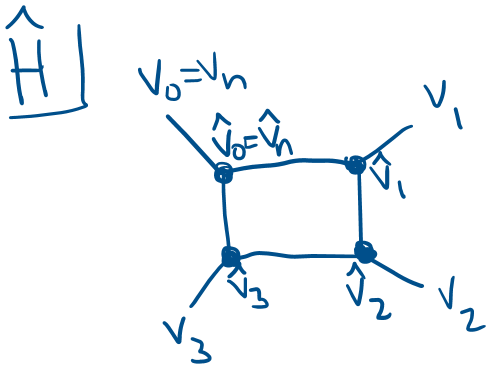
\includegraphics[width=.35\textwidth]{hdak.png}
        \caption{The graph $\hat H$.} \label{fig:hdak}
    \end{figure}

    Let the vertices on cycle $H$ be $v_0, v_1, \dots, v_n = v_0$.
    Then the subproblem is defined in the following way: let $C[i, j, h(i), h(j)]$ be the minimum cost of only the part from $i$ to $j$ in $H$ (clockwise), where $\hat v_i$ is mapped to $h(i)$ and $\hat v_j$ is mapped to $h(j)$.
    Here, $0 \le i < j \le n$ and all terminals must be mapped to itself.

    If $j = i + 1$, then the cost is $b_i \cdot d_c(v_i, h(i)) + d_{ij} \cdot d_c(h(i), h(j)) + b_j \cdot d_c(v_j, h(j))$.
    Here, $d_c(u, v)$ is the shortest path under cost function $c$ from $u$ to $v$ in $G$, i.e.\ buying each edge on the shortest path once.
    It is considers the edge $\{\hat v_i, \hat v_j\}$ in the cycle in $\hat H$ and the two edges between these nodes and the corresponding terminals.
    Because we required the capacities to be minimal, we know that there exist valid demands that utilize the full capacity.
    Thus, we must buy these.

    If $j$ is not $i+1$, we pick a node $\hat v_k$ with $i < k < j$ (for example, $k = i + 1$).
    Then, $C[i, j, h(i), h(j)]$ is the minimum over all possible mappings $h(k) \in V_G$ of $C[i, k, h(i), h(k)] + C[k, j, h(k), h(j)] - b_k d(v_k, h(k))$.
    Both parts consider the edge $(v_k, \hat v_k)$, so we should remove it once to obtain the correct answer.
    See also Figure~\ref{fig:dp} for a sketch of the situation.

    \begin{figure}
        \centering
        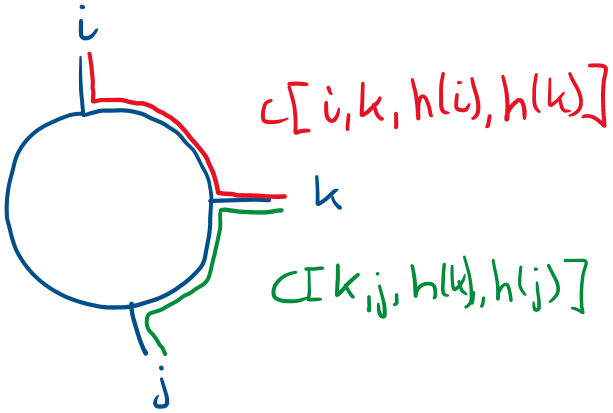
\includegraphics[width=.35\textwidth]{dp.png}
        \caption{Sketch of the situation for the dynamic program (in $\hat H$).} \label{fig:dp}
    \end{figure}

    This leads to the following recurrence:
    \[
        C[i, j, h(i), h(j)] = \begin{cases}
                                  0 &\text{if $i \ge j$} \\
                                  b_i \cdot d_c(v_i, h(i)) + d_{ij} \cdot d_c(h(i), h(j)) + b_j \cdot d_c(v_j, h(j)) &\text{if $j = i+1$}\\
                                  \displaystyle \min_{h(k) \in V_G} \{ C[i, k, h(i), h(k)] + C[k, j, h(k), h(j)] - b_k d(v_k, h(k)) \} &\text{otherwise}\\


        \end{cases}
    \]

    We can now determine all values by first determining the base cases, then all valid intervals of length two, then length three etc.
    The last interval will go from $0$ to $n$ and this is the interval we are interested in.
    The minimum over all mappings $h(0)$ of $C[0, n, h(0), h(0)]$ will be the minimum cost.
    The actual mappings can be obtained by searching the table backwards.


\end{document}
